\section{Approach to fault tolerance in spacecrafts}

The characteristics of space exploration missions have always required
innovative fault management (FM) strategies\footnote{The term \textit{Fault
Management} is often used interchangeably with the term \textit{Fault
Protection} in NASA documentation.} in order to achieve mission success.
The used FM strategies and implementations vary significantly from mission to
mission, but there are a set of general characteristics that influence the
design of the FM. Engineers from NASA have been working on a Fault Management
Handbook with the purpose of being \textit{`a guidance document to provide
guidelines and recommendations for defining, developing, analyzing, evaluating,
testing, and operating the Fault Management (FM) element of flight
systems`}\cite{nasa-fm-handbook}.
 
According to \cite{nasa-fm-handbook}, a space missions FM engineer has the role
of analysing mission attributes and characteristics and defining FM
requirements, as well as developing hardware and software architectures that
provide fault protection and assure the success of missions. This process is
ilustrated in Figure~\ref{fig:fm_design}.

\begin{figure}[htb] 
	\begin{center}
	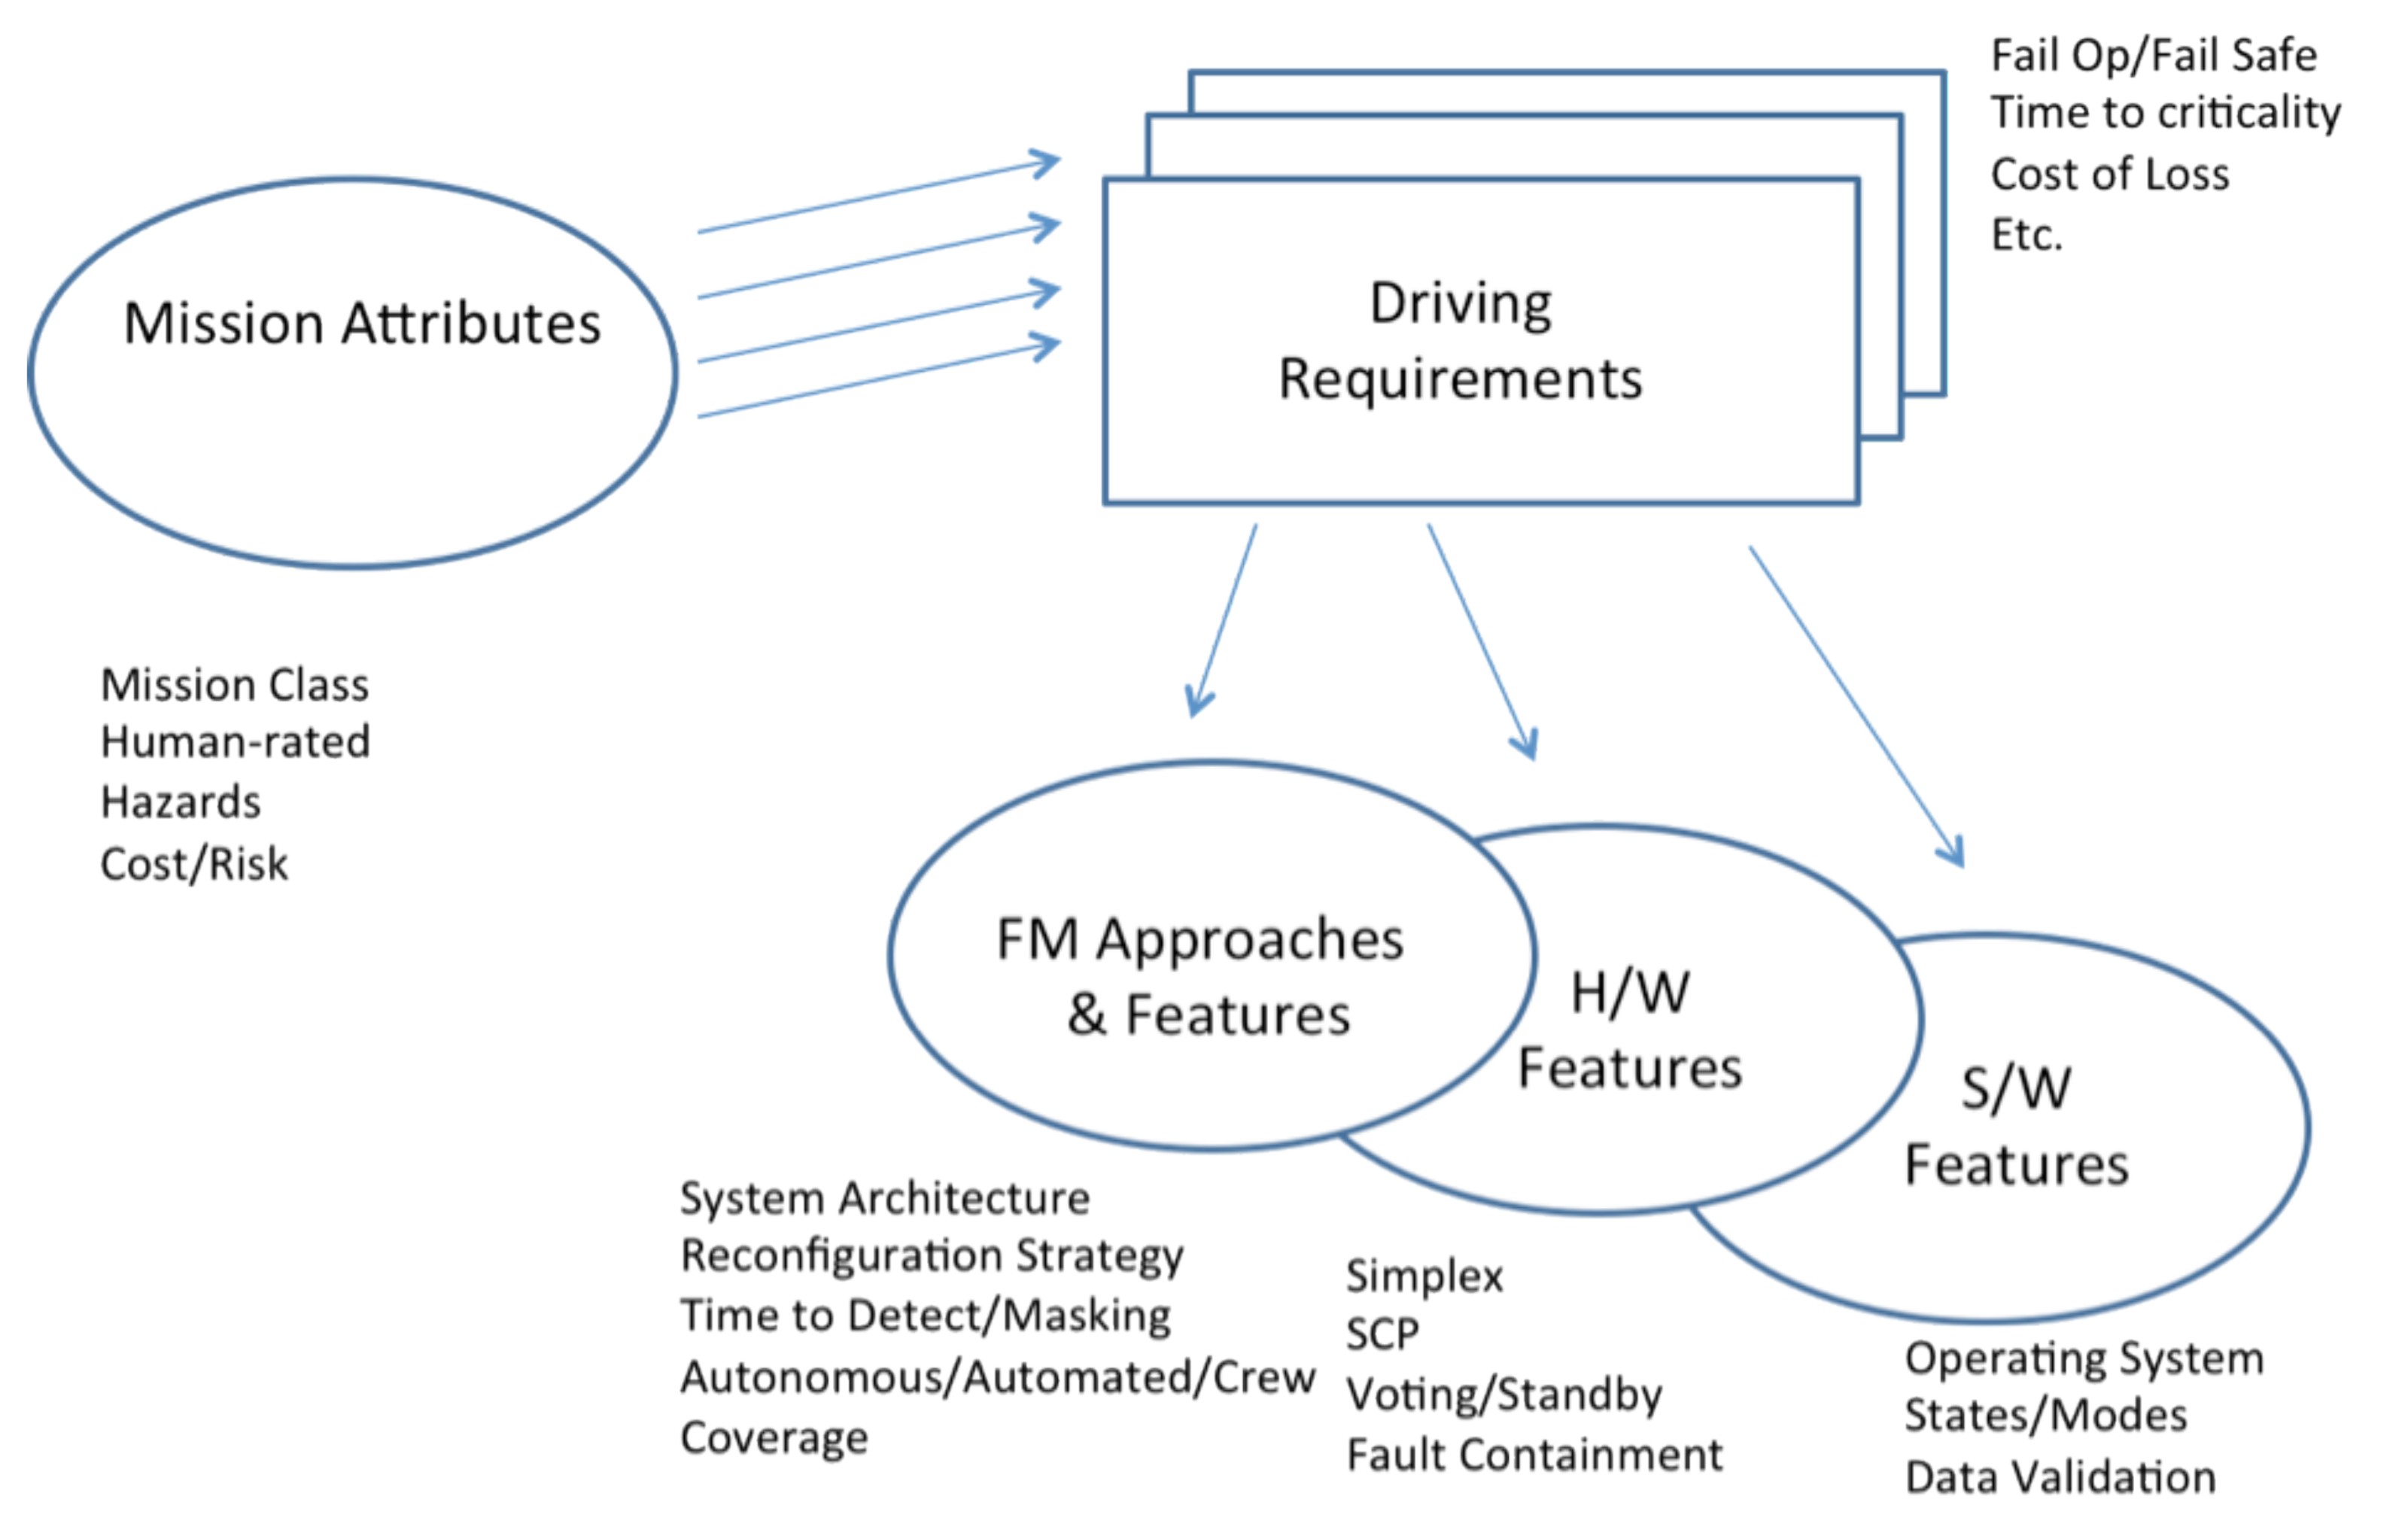
\includegraphics[width=0.8\textwidth]{img/fm_design.png}
	\caption{Fault Management design process. \small{\textit{Source: NASA Fault
	Tolerance Handbook, draft 2, 2012}}}
	\label{fig:fm_design}
	\end{center}
\end{figure}

The first step during development of the FM for a space mission is a clear
identification of mission goals and of functions and resources that are critical
and need to be protected\footnote{These include functions, resources, events
which are needed to achieve the mission's goals. E.g.: successful launch,
scientific payload, collected data etc. }. Subsequently, the FM engineers need
to perform an analysis of the system architecture to identify the mission
characteristics which are definitory for the fault protection functions. Fault
management will need to be implemented throughout the system, however they need
to take into account restrictions enforced by the mission characteristics. For
example, in the case of deep space exploration mission, which have delayed and
infrequent contact with the mission command on Earth, or during time critical
steps of missions (e.g. planetary atmospheric entry), fault management
\textbf{response latency} is critical. According to the NASA Fault Management
Handbook \cite{nasa-fm-handbook}, response latency is \textit{'the time from the
occurrence of a fault to the correction of the failure condition'} and is
\textit{'built from the various mission and system characteristics that impact
the execution of each of the core FM functions'}. To assure system reliability,
the FM response needs to either clear or contain the effects of a failure before
the failure is propagated to other components or before system issues occur.

The next step followed by the FM engineers is to design and implement software
and hardware solutions to assure the fault protection of a spacecraft. A series
of techniques can be used in different situations and at different moments of
time (different stages). In the presentation of Fault Management at the Jet
Propulsion Lab\cite{fm-jpl}, John Day and Michel Ingham detail a hierarchy of
approaches and give examples of a series of strategies that may be used to
assure fault protection. The hierarchy can be seen in
Figure~\ref{fig:fault_protection_hierarchy}. A first strategy that should be
followed is to to avoid faults altogether, through \textbf{fault avoidance}
techniques. However, for cases when faults do occur, \textbf{fault tolerance}
needs to be in place, to assure that any faults have minimal effects on the ship
and do not cause a mission failure. From this category, for example,
\textbf{Fault Masking}, \textbf{Gradual Degradation} and \textbf{Fault
Detection, Isolation and Recovery} (FDIR) are some general strategies that can
be employed.

\begin{figure}[htb]
	\begin{center}
	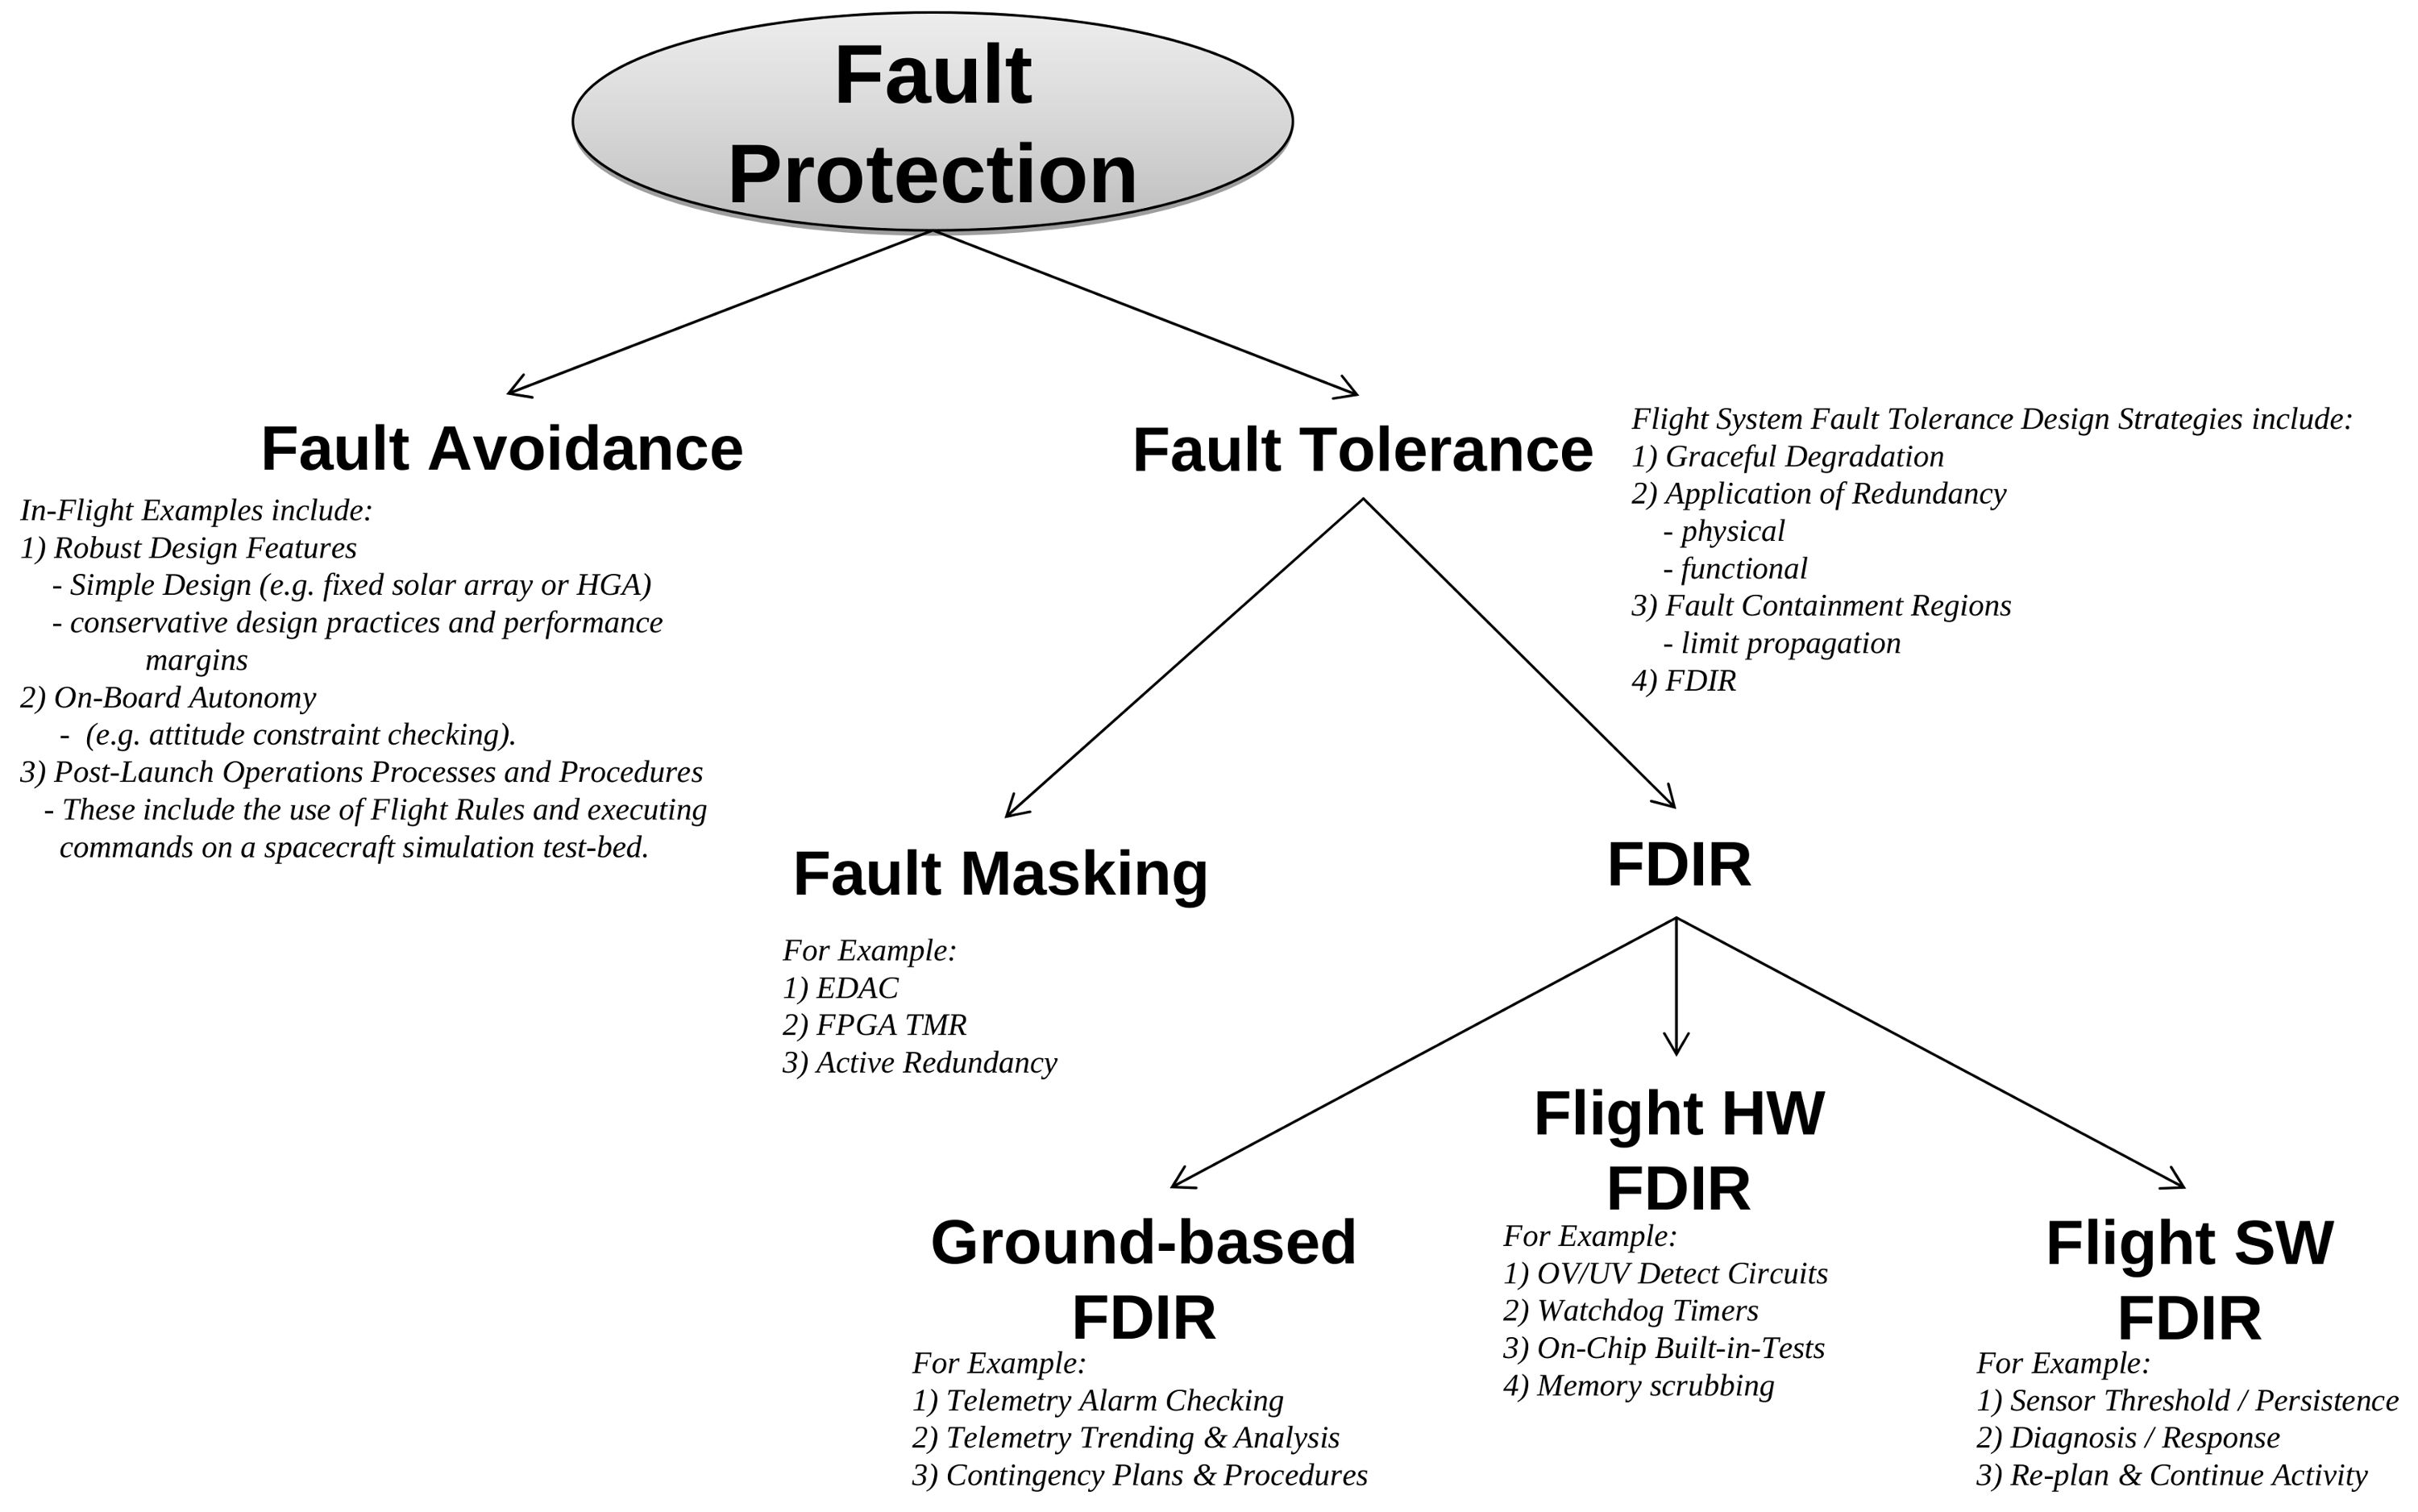
\includegraphics[width=0.9\textwidth]{img/fault_protection_hierarchy.png}
	\caption{Fault protection general hierarchy. \small{\textit{Source: J.
	Day and M. Ingham, Fault management at JPL: past, present and future, 2011}}}
	\label{fig:fault_protection_hierarchy}
	\end{center}
\end{figure}

The design and implementation of FM needs to be followed by Verification and
Validation, to prove that the system complies with the system requirements and
that the response to failures is the intended one. Besides the mission specific
requirements, all space missions have to respect some general safety
requirements. Mandatory ones include the \textbf{NASA General Safety Program
Requirements} (NPR-8715.3) and the \textbf{Eastern and Western Range Safety
Requirements} (EWR 127.1)\footnote{EWR-127.1 represents the specification of
safety requirements for the launch site. It is being replaced with the
\textbf{Air Force Space Command Manual Range Safety User Requirements(AFSCPCMAN
91-710).}}. In addition, a multitude of other documents include recommendations
for requirements related to fault protection in the case of spacecrafts. Some
examples include: Rules for the Design, Development, Verification, and Operation
of Flight Systems (GSFC-STD-1000E), NASA Systems Engineering Processes and
Requirements (NPR 7123.1A), Risk Classification for NASA Payloads (NPR 8705.4)
etc.

\todo{Include the execution architecture and some text from JPL.}
\begin{figure}[htb]
	\begin{center}
	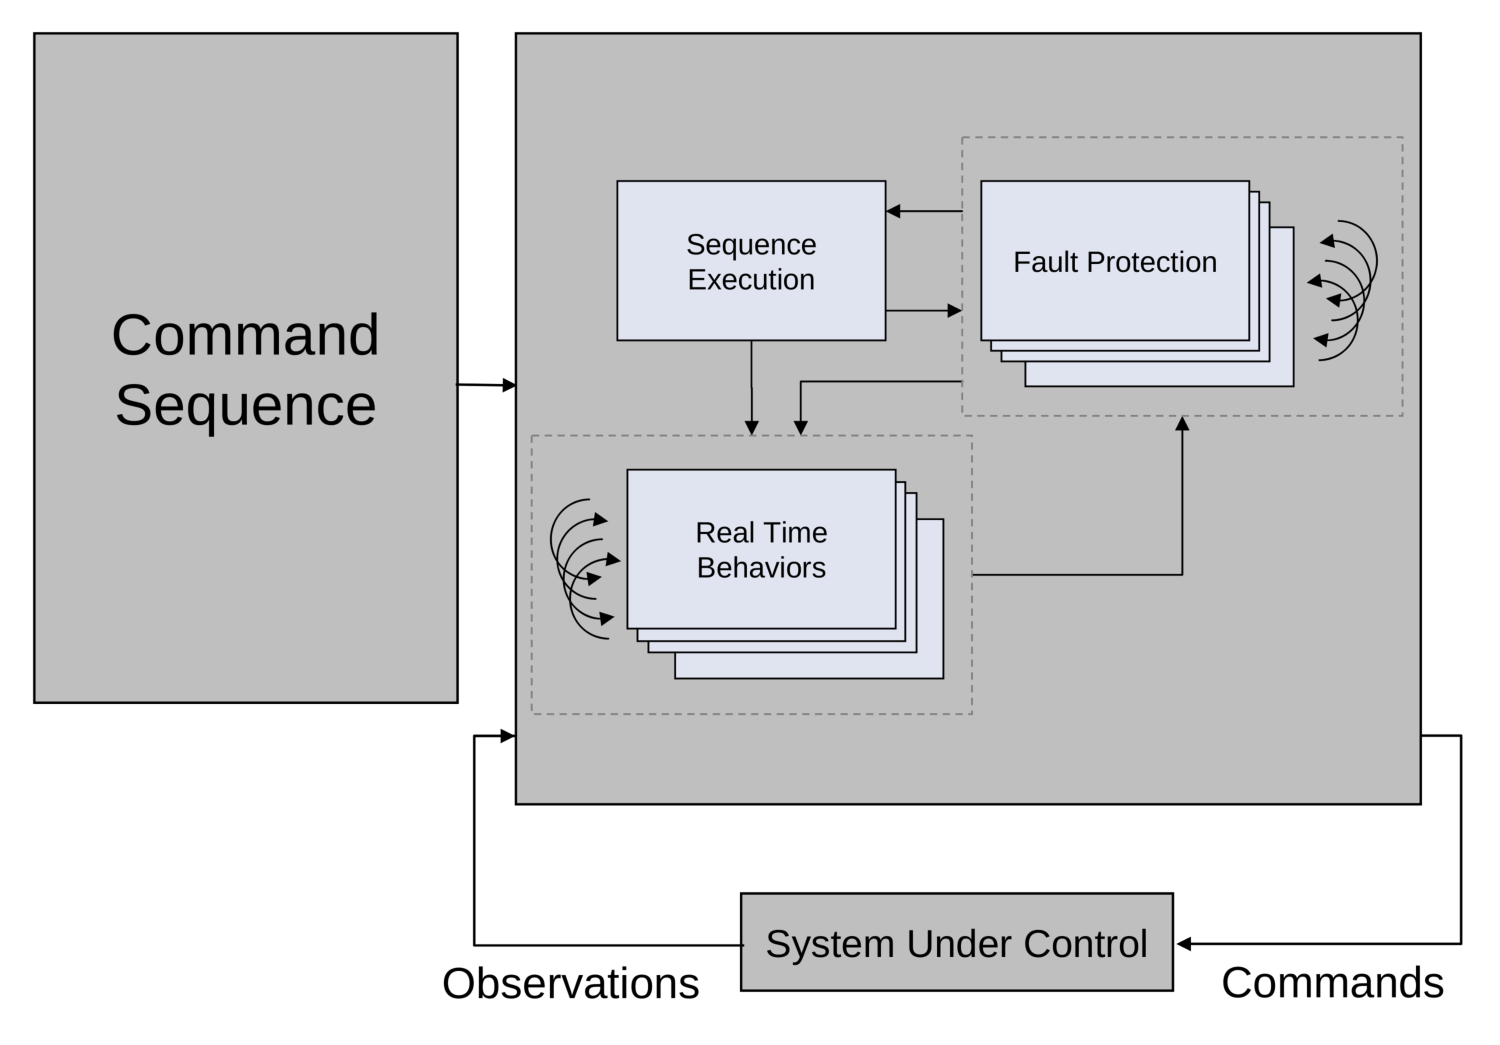
\includegraphics[width=0.6\textwidth]{img/spacecraft_execution_architecture.pdf}
	\caption{Typical Spacecraft Execution Architecture. \small{\textit{Source: J.
	Day and M. Ingham, Fault management at JPL: past, present and future, 2011}}}
	\label{fig:spacecraft_execution_architecture}
	\end{center}
\end{figure}